\documentclass[11pt]{article}
\usepackage[margin=1in]{geometry}
\usepackage{amsmath,booktabs,graphicx,hyperref}
\graphicspath{{../results/}}

\title{What Does Entanglement Buy a Quantum RL Policy?\\
\large Representational similarity of PQC and MLP policies across entangling depth}
\author{Shushant}
\date{October 2026}

\begin{document}
\maketitle

\begin{abstract}
We train PPO agents whose actor is a parameterised quantum circuit (PQC) with entangling depth
$k\in\{0,\dots,4\}$ (CZ entanglers after the first $k$ of $L=4$ variational layers; \texttt{chain} and
all-to-all topologies, identical parameter count). We compare their pre-measurement representations
with a classical MLP using representational similarity analysis (RSA) and linear CKA, with noise ceilings
and a hierarchical bootstrap. The study was pre-registered: three hypotheses and three gates.
The reliability gate failed: two seeds of the same circuit can agree with each other at RSA as low as 0.19.
Representational reliability is therefore our headline result. Neither the depth trend in similarity to the MLP (H1)
nor its coincidence with return saturation (H2) replicates across tasks: H1 is supported only on
Acrobot \texttt{chain}, and only weakly. Circuits with no entanglers do differ from the MLP more on coupled
degrees of freedom (H3). This is clearly the case on Pendulum (10/10 \texttt{chain} seeds significant)
but not on CartPole. Gradient variance at initialisation falls with depth on every task.
All experiments are exact classical simulations of 3--6 qubits.
\end{abstract}

\section{Setup}
\paragraph{Policies.} Quantum actor: $n=$ observation-dimension qubits, $L=4$ layers of RY/RZ rotations, with
data re-uploading through trainable input scaling. CZ entanglers follow the first $k$ layers. The representation is
$\langle Z_i\rangle$, and the ablation adds $\langle Z_iZ_j\rangle$. Classical baselines: the primary MLP
(obs$\to$64$\to n$, tanh), which matches representation width and range, and \texttt{mlp-pm}, which is parameter-matched ($\pm10\%$).
Heads and the critic are identical across families.
\paragraph{Training.} CleanRL-style PPO with hyperparameters frozen after a three-round CartPole pilot
(actor LR $5\times10^{-4}$, quantum $5\times10^{-3}$, critic $2.5\times10^{-3}$). Tasks: CartPole-v1 (500k steps),
Pendulum-v1, and Acrobot-v1. Each task has 9 quantum conditions $\times$ 5 seeds plus 2 MLPs, with seeds extended to 10 for
\texttt{q-sep-k0}, \texttt{q-chain-k4} and \texttt{mlp}. That gives 70 runs per task, all of which completed.
\paragraph{Analysis.} 500 probe states are pooled from rollouts of all trained runs, with an equal share per run.
We use correlation-distance RDMs and Spearman RSA. The noise ceiling is the mean between-seed RSA, and
$\mathrm{RSA_{norm}} = \mathrm{RSA}(q,c)/\sqrt{\mathrm{ceil}_q\,\mathrm{ceil}_c}$. CIs come from a hierarchical bootstrap
(seeds, then probes; 2000 resamples). H1 is Spearman$(k,\mathrm{RSA_{norm}})$, and H2 is a two-segment
breakpoint fit. H3 is a permutation test on separable-minus-MLP RDM discrepancy for coupled versus magnitude-matched uncoupled probe pairs.

\section{Gates}
\begin{tabular}{lll}\toprule
G1 & E1 measurement validation (synthetic RSA/CKA, statevector oracle) & PASS\\
G2 & quantum PPO solves CartPole ($\geq475$ in $\geq3/5$ seeds, $k=0,4$) & PASS (5/5, 5/5)\\
G3 & quantum seed-to-seed RSA ceiling $\geq 0.2$ & \textbf{FAIL} (CartPole \texttt{q-all-k3}: 0.191)\\\bottomrule
\end{tabular}

\noindent The Pendulum fallback was also triggered: \texttt{q-sep-k0} reached $-400$ in 0/5 seeds. Pendulum
is therefore used only for H3, and Acrobot is the second depth-curve task.

\section{Results}
\subsection{Reliability (headline)}
\begin{tabular}{lcc}\toprule
Task & quantum ceilings & primary MLP ceiling\\\midrule
CartPole & 0.19--0.60 & 0.49\\
Pendulum & 0.27--0.58 & 0.73\\
Acrobot & 0.26--0.76 & 0.84\\\bottomrule
\end{tabular}

\noindent The lowest ceilings belong to deep all-to-all circuits. Independently trained copies of the same
circuit often share less representational geometry than they share with an MLP. Any between-family
comparison inherits this noise.

\subsection{Hypotheses}
\begin{tabular}{llll}\toprule
 & CartPole & Acrobot & Pendulum\\\midrule
H1 & inconclusive & \texttt{chain} supported [0.1, 1.0]; \texttt{all} inconclusive & ---\\
H2 & not supported & \texttt{chain} supported; \texttt{all} not & ---\\
H3 & not supported (3/10, 2/5) & 8/10, 3/5 seeds; small $T$ & \textbf{supported} (10/10, 4/5; $T\approx0.06$)\\\bottomrule
\end{tabular}

\noindent On CartPole the return axis is saturated: nearly every condition reaches 500, so H2 has no
breakpoint to match. The Acrobot \texttt{chain} support comes mainly from $k=4$, since RSA$_{\text{norm}}$ is flat at
0.82--0.87 for $k\le3$. CKA agrees in direction with RSA everywhere.

\begin{figure}[h]\centering
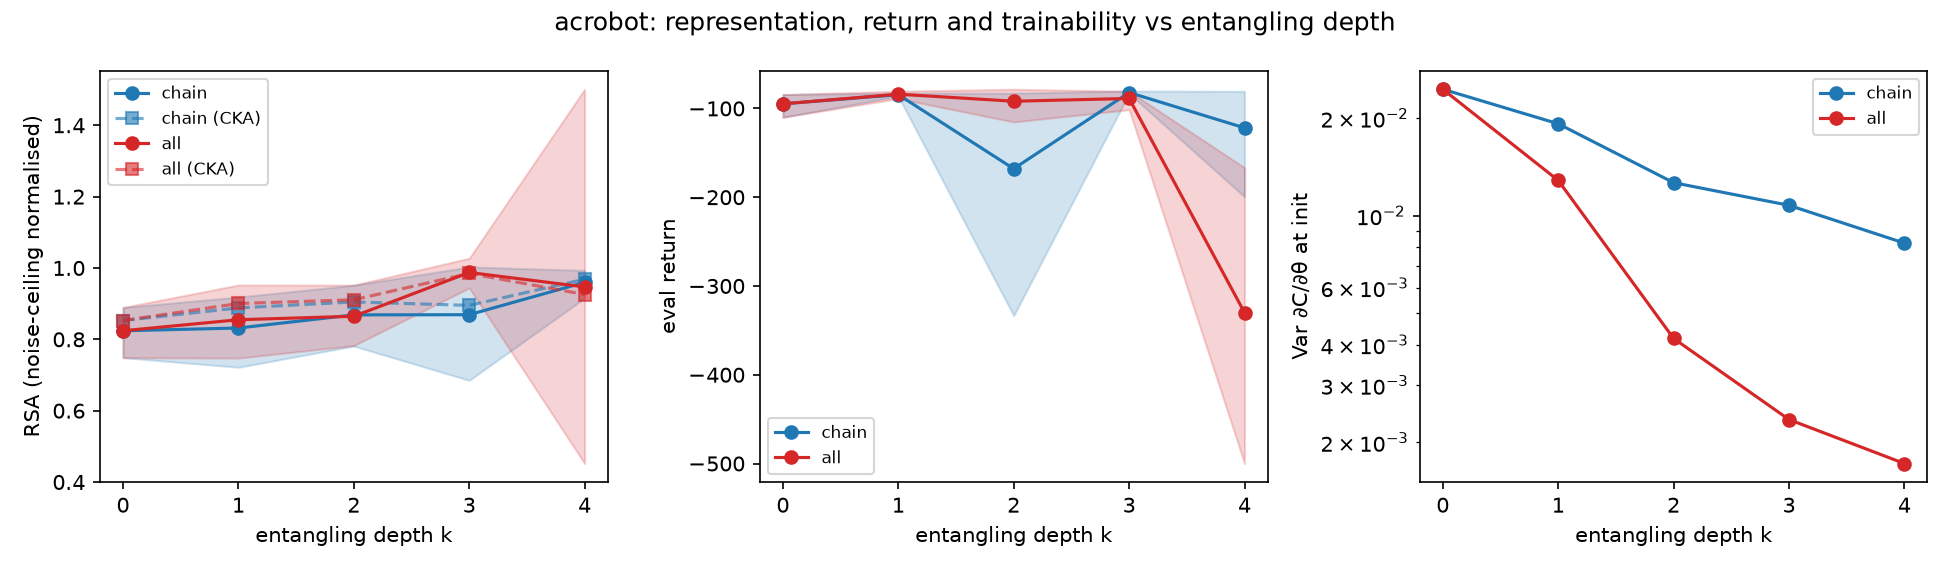
\includegraphics[width=.48\linewidth]{acrobot/rsa_return_gradvar_curve.png}
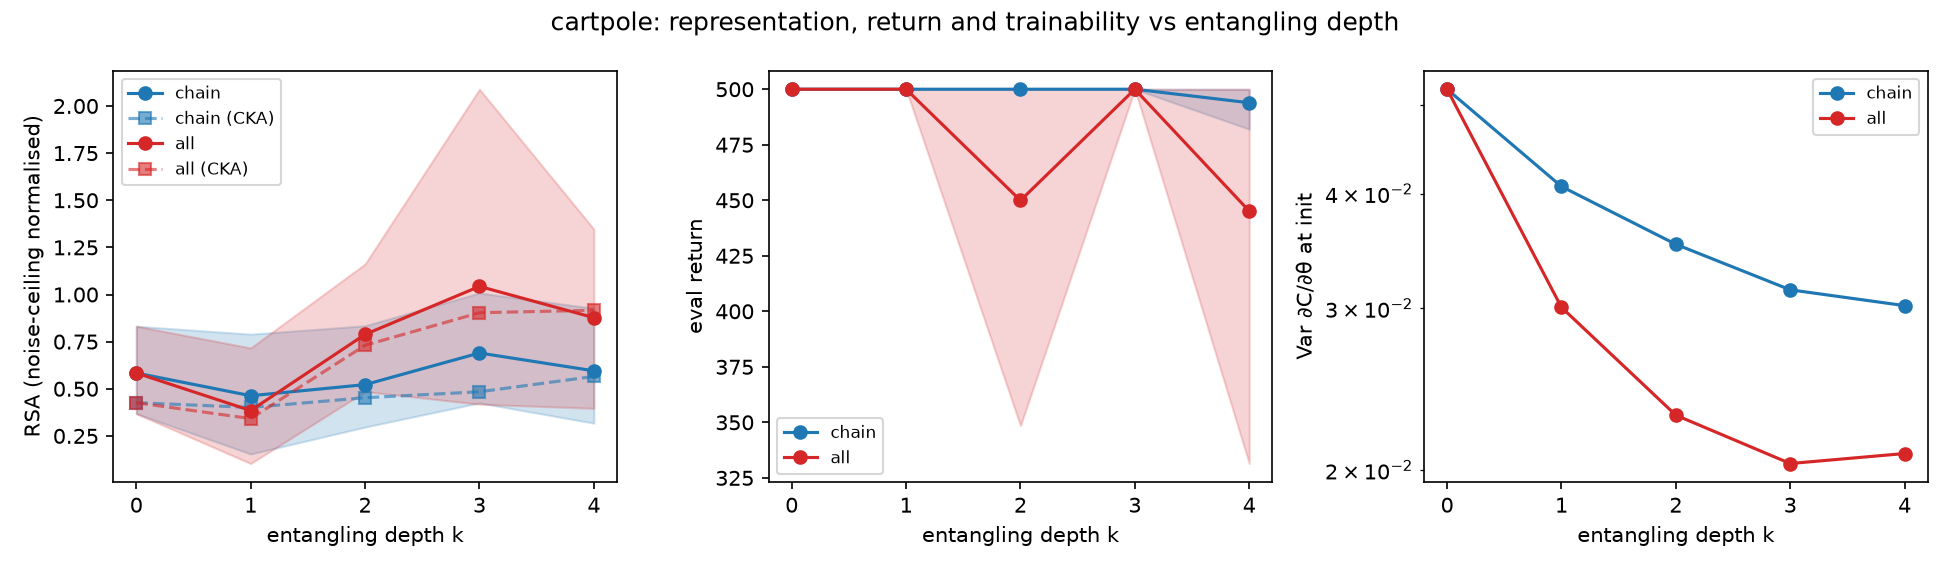
\includegraphics[width=.48\linewidth]{cartpole/rsa_return_gradvar_curve.png}
\caption{RSA$_{\text{norm}}$, return and initial gradient variance against entangling depth (left: Acrobot; right: CartPole).}
\end{figure}

\begin{figure}[h]\centering
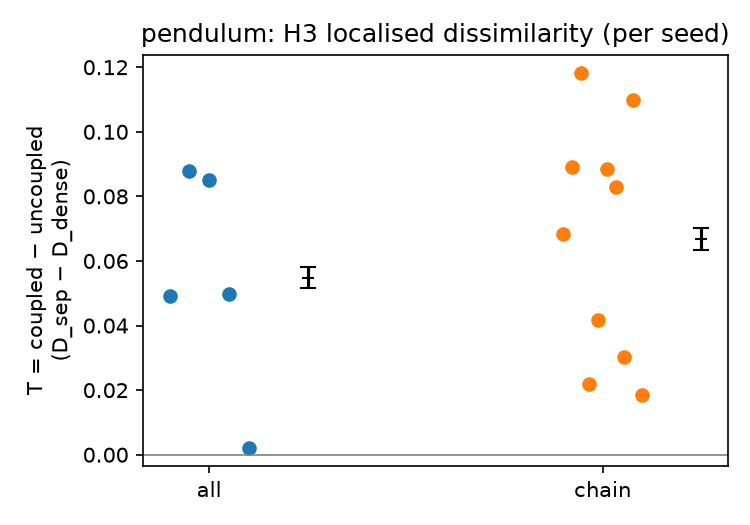
\includegraphics[width=.6\linewidth]{pendulum/partitioned_dissimilarity.png}
\caption{Pendulum H3: separable-minus-MLP discrepancy on coupled versus uncoupled probe pairs.}
\end{figure}

\subsection{Trainability}
Mean gradient variance over 200 random initialisations falls monotonically with depth on all tasks, and falls faster for
all-to-all. For example, on Acrobot it is 0.025 at $k=0$, 0.008 for \texttt{chain} $k=4$ and 0.002 for \texttt{all} $k=4$.

\subsection{Exploratory}
Under the frozen hyperparameters, only circuits with $k\ge3$ (and \texttt{q-all-k2}) solve Pendulum
($\approx-150$). Shallow circuits and the primary MLP fail ($-629\pm145$). The hyperparameters were tuned on
CartPole, so this is not evidence of a quantum advantage. On CartPole, the observable ablation ($\langle Z\rangle+\langle ZZ\rangle$)
lowers RSA$_{\text{norm}}$ at every depth but keeps the positive point trend. The probe ablation is stable from 200 to 1000 probes.

\section{Limitations}
These are exact simulations with no hardware noise, on small systems with five depth points.
There is one entangler family (CZ), and hyperparameters were tuned only on CartPole. The Pendulum reference policy does
not solve the task, and the qubit count differs between tasks. See \texttt{LIMITATIONS.md}.

\section{Reproducibility}
\texttt{scripts/reproduce.sh} runs G1, then the three sweeps (with the fallback check), the ablations, the analysis and the gates.
Completed runs are skipped. The full run takes about 12 h on 16 CPU workers.

\end{document}
